%  $
% \newcommand{\MtdFull}[1]{\frac{D \, #1}{D \, t}}
% \newcommand{\Pd}[2]{\frac{\partial #1}{\partial #2}}
% \newcommand{\d}{\text{d} }
% \newcommand{\Dd}[2]{\frac{\d #1}{\d #2}}
% \newcommand{\dt}[1]{#1 ^{\bullet}}
% \newcommand{\dV}{\; \text{d}V}
% \newcommand{\dA}{\; \text{d}A}
% \newcommand{\dx}{\; \text{ d}x}
% \newcommand{\dy}{\; \text{ d}y}
% \newcommand{\dz}{\; \text{ d}z}
% \newcommand{\dxi}{\; \text{ d}\xi}
% \newcommand{\deta}{\; \text{ d}\eta}
% \newcommand{\dzeta}{\; \text{ d}\zeta}
% \newcommand{\grad}[1]{\text{grad}\left(#1\right)}
% \renewcommand{\div}[1]{\text{div} \left(#1\right)}
% \newcommand{\td}[1]{\dot{#1}}
% \newcommand{\tdd}[1]{\ddot{#1}}
% \newcommand{\T}{\rp{T}}
% \newcommand{\rp}[1]{^{\text{#1}}}
% \newcommand{\rs}[1]{_{\text{#1}}}
% \renewcommand{\bm}[1]{\boldsymbol{#1}}
% \newcommand{\e}{\epsilon}
% \newcommand{\eb}{\bm{\e}}
% \newcommand{\s}{\sigma}
% \newcommand{\sb}{\bm{\sigma}}
% $

\subsubsection{Die Balken-FEM}

\begin{figure}[!htbp]
\centering
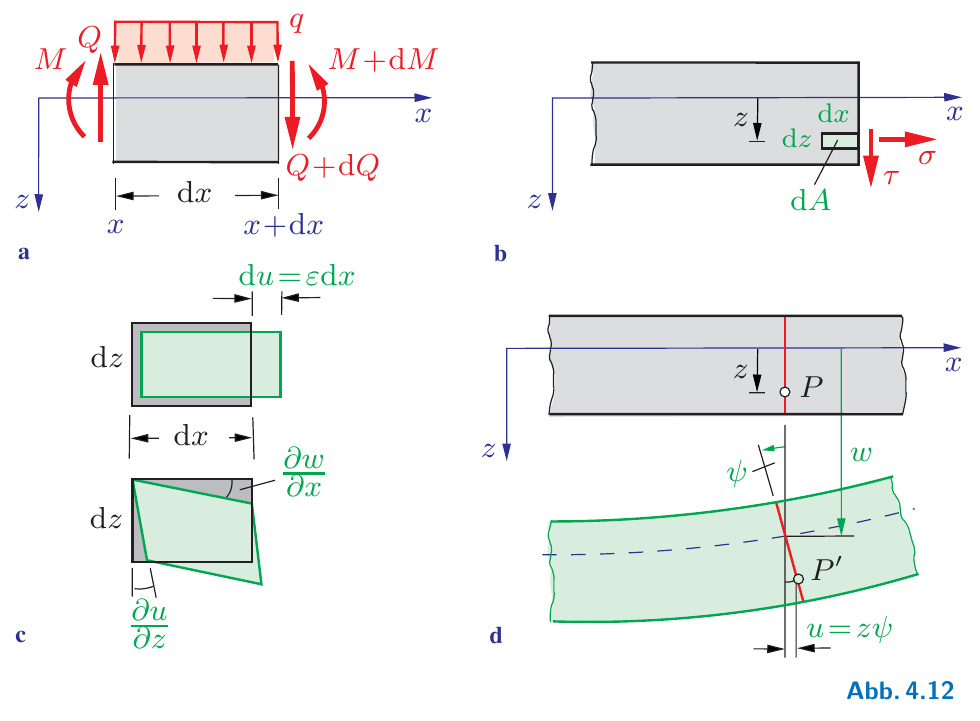
\includegraphics[width=0.7\linewidth]{files/Balken_TM2-047a15c5c31955daed71737e695a57f6.png}
\caption[]{Schnittgrö$\beta$en und Kinematik am Balkenelement nach \cite{gross2007technische}}
\label{balken02}
\end{figure}

Als weiteren Vertreter der Strukturelemente innerhalb der Finite-Elemente-Methode (FEM) betrachten wir im Folgenden die Balken-FEM. Die Impulsbilanz des Euler-Bernoulli-Balkens ist eine Differentialgleichung 4. Ordnung. Unter der Voraussetzung einer konstanten Biegesteifigkeit $EI_y$ lautet diese:

\begin{equation}
\label{balkendglsimple_2}
  w^{IV} =  \frac{q(x)}{E I_y} \; .
\end{equation}
Die obige \textbf{starke Form} der Balken-DGL wird im Folgenden in eine \textbf{schwache Form} umgewandelt. Formal wird die Differentialgleichung wieder mit einer beliebigen Testfunktion $\delta w$ multipliziert und über den Balken integriert. Die schwache Form lautet dann:

\begin{equation}
\label{weakBalken_01}
  EI_y \int_L \delta w'' w'' \dx - \int_L q(x) \delta w \dx - F_I \delta w_I - M_J \delta w'_J = 0 \; .
\end{equation}

Hierbei stellen $F_I$ und $M_I$ die an den Knoten angreifenden Einzellasten und Momente dar. Es ist zu beachten, dass die zweite Ableitung der Durchbiegung die höchste Ableitungsordnung in dieser Variationsgleichung darstellt. Für die Finite-Elemente-Approximation müssen ($C^1$)-stetige Ansatzfunktionen formuliert werden. Dies impliziert, dass an den Knotenpunkten die Verschiebungsansätze sowohl in der Durchbiegung ($w$) als auch in der Neigung ($w'$) stetig sein müssen. Anders als beim Stabelement sind die Freiheitsgrade an den Knotenpunkten nicht nur die Verschiebungen, sondern auch die Neigungen. Dies ist charakteristisch für die Formulierung von Balkenelementen, aber auch für die Formulierung von Plattenelementen und Schalenelementen.

%  -+-+-+-+-+-+-AI-SPLIT

\paragraph{Ansatzfunktionen}

\begin{figure}[!htbp]
\centering
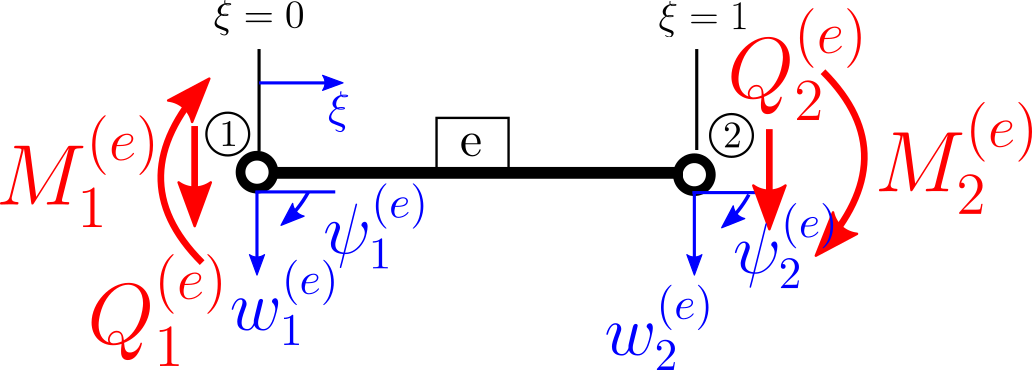
\includegraphics[width=0.7\linewidth]{files/Balkenelement-a8a2414933a947e716e92a521cf26529.png}
\caption[]{Balkenelement mit lokalen Freiheitsgraden}
\label{balken03_1}
\end{figure}

Analog zum Stabelement führen wir die normierte Koordinate $\xi=\frac{x}{\ell_e}$ ein. Die Ansatzfunktionen für die Durchbiegung $w_h$ werden dann als Linearkombination der Formfunktionen $N_I$ und der Freiheitsgrade $w_I$ geschrieben:

\begin{align}
  w_h & = N_1(\xi) w_1 + N_2(\xi) \psi_1 \ell_e +  N_3(\xi) w_2 + N_4(\xi) \psi_2 \ell_e = \sum_{I=1}^{4} N_I(\xi) w_I \\
  & = \begin{pmatrix} N_1(\xi) & N_2(\xi)\ell_e & N_3(\xi) & N_4(\xi)\ell_e \end{pmatrix} \begin{pmatrix} w_1 \\ \psi_1 \\ w_2 \\ \psi_2 \end{pmatrix}
\end{align}

Der Vektor der Freiheitsgrade $\bm{w}=w_I$ enthält die Durchbiegung $w$ und die Neigung $\psi$ an den beiden Knoten des Balkenelements. Wie bei den Formfunktionen des Stabelements ist die Formfunktion $N_I$ nur für den Freiheitsgrad $w_I$ identisch mit 1 und für alle anderen Freiheitsgrade gleich 0. Formfunktionen, die diese Eigenschaft haben, sind zum Beispiel die Hermite-Polynome:
\begin{align}
  \bm{N} = \begin{pmatrix} 
  1-3\xi^2+2\xi^3 \\ 
  (\xi-2\xi^2+\xi^3)\ell_e \\ 
  3\xi^2-2\xi^3 \\ 
  (-\xi^2+\xi^3)\ell_e \end{pmatrix}
\end{align}

%  
% ```{code-cell} ipython3
% ---
% mystnb:
%   figure:
%     caption: Formfunktionen für ein Balkenelelement mit Hermite-Interpolation.
%     name: Shape-Beam
% tags: [
%   "remove-input"
%   ]
% ---
% import numpy as np
% import plotly.graph_objects as go
% 
% # Define the x values
% x = np.linspace(0, 1, 100)
% 
% # Define the shape functions - Hermite polynomials 4th order
% N1 = 1 - 3*x**2 + 2*x**3
% N2 = x - 2*x**2 + x**3
% N3 = 3*x**2 - 2*x**3
% N4 = -x**2 + x**3
% 
% # Create the figure
% fig = go.Figure()
% 
% # Add traces for each shape function
% fig.add_trace(go.Scatter(x=x, y=N1, mode='lines', name='N_1'))
% fig.add_trace(go.Scatter(x=x, y=N2, mode='lines', name='N_2'))
% fig.add_trace(go.Scatter(x=x, y=N3, mode='lines', name='N_3'))
% fig.add_trace(go.Scatter(x=x, y=N4, mode='lines', name='N_4'))
% 
% # Update layout with LaTeX math
% fig.update_layout(
%     xaxis_title=r'$\eta$',
%     yaxis_title=r'$N(\eta)$',
%     legend=dict(x=1.05, y=1),
%     font=dict(family="Serif", size=15),
%     template='plotly_white',
%     xaxis=dict(showgrid=True, gridcolor='grey', gridwidth=0.6, griddash='dash'),
%     yaxis=dict(showgrid=True, gridcolor='grey', gridwidth=0.6, griddash='dash')
% )
% 
% # Show the plot
% # fig.show()
% ```

\begin{framed}
\textbf{Wichtige Eigenschaften des Ansatzes des Balkens}\\
\begin{itemize}
\item Die Durchbiegung $w$ ist $C^1$-stetig.
\item Die Durchbiegung $w$ und die Neigung $\psi=w'$ sind über die Elementgrenzen hinweg stetig.
\item Durch die Wahl der Formfunktionen haben die Knotenfreiheitsgrade die Bedeutung von Durchbiegung und Neigung.
\end{itemize}
\end{framed}

Auch für die Testfunktion $\delta w$ wird der Ansatz (\ref{Ansatz_Balken}) verwendet.

%  -+-+-+-+-+-+-AI-SPLIT

\paragraph{Elementsteifigkeitsmatrix (Diskretisierung Term 1 in Gleichung (\ref{weakBalken_01}) )}

Eingesetzt in die schwache Form liefert der erste Term die Elementsteifigkeitsmatrix. Hierfür müssen zunächst die Ableitungen des Ansatzes bzgl. $x$ berechnet werden. Aus
$\dx = \ell_e \dxi$ folgt:
\begin{align}
  \Dd{w}{x} & = \frac{1}{\ell_e} \Dd{w}{\xi} = \frac{1}{\ell_e} \bm{N}_{,\xi} \bm{w} \\
  \Dd{^2 w}{x^2} & = \frac{1}{\ell_e^2} \Dd{^2 w}{\xi^2} = \frac{1}{\ell_e^2} \bm{N}_{,\xi\xi} \bm{w}
\end{align}

Eingesetzt in die schwache Form ergibt sich für die Elementsteifigkeit:

\begin{align}
  & \delta \bm{w}^T \frac{EI}{\ell^3_e} \int_0^{1}  \bm{N}_{,\xi\xi}^T \bm{N}_{,\xi\xi} \dxi\, \bm{w} \\
  &= \delta \bm{w}^T \frac{EI}{\ell^3_e} \int_0^{1} \begin{pmatrix}
    12\xi -6 & (6\xi-4)\ell_e  & -12\xi+6 & (6\xi-2)\ell_e 
  \end{pmatrix} \begin{pmatrix}
    12\xi -6 \\
    (6\xi-4)\ell_e  \\
    -12\xi+6 \\
    (6\xi-2)\ell_e 
  \end{pmatrix} \dxi\, \bm{w} \\
  &= \delta \bm{w}^T \frac{EI}{\ell^3_e} \int_0^{1} \begin{pmatrix}\left(12 \xi - 6\right)^{2} & \ell_e \left(6 \xi - 4\right) \left(12 \xi - 6\right) & \left(6 - 12 \xi\right) \left(12 \xi - 6\right) & \ell_e \left(6 \xi - 2\right) \left(12 \xi - 6\right)\\\ell_e \left(6 \xi - 4\right) \left(12 \xi - 6\right) & \ell_e^{2} \left(6 \xi - 4\right)^{2} & \ell_e \left(6 - 12 \xi\right) \left(6 \xi - 4\right) & \ell_e^{2} \left(6 \xi - 4\right) \left(6 \xi - 2\right)\\\left(6 - 12 \xi\right) \left(12 \xi - 6\right) & \ell_e \left(6 - 12 \xi\right) \left(6 \xi - 4\right) & \left(6 - 12 \xi\right)^{2} & \ell_e \left(6 - 12 \xi\right) \left(6 \xi - 2\right)\\\ell_e \left(6 \xi - 2\right) \left(12 \xi - 6\right) & \ell_e^{2} \left(6 \xi - 4\right) \left(6 \xi - 2\right) & \ell_e \left(6 - 12 \xi\right) \left(6 \xi - 2\right) & \ell_e^{2} \left(6 \xi - 2\right)^{2}\end{pmatrix} \dxi\, \bm{w} \\
  &= \delta \bm{w} \underbrace{\frac{EI}{\ell^3} \begin{pmatrix}12 & 6 \ell_e & -12 & 6 \ell_e\\6 \ell_e & 4 \ell_e^{2} & - 6 \ell_e & 2 \ell_e^{2}\\-12 & - 6 \ell_e & 12 & - 6 \ell_e\\6 \ell_e & 2 \ell_e^{2} & - 6 \ell_e & 4 \ell_e^{2}\end{pmatrix}}_{\bm{K_e}} \,  \bm{w}
\end{align}

\paragraph{Diskretisierung der Streckenlast}

Die Streckenlast $q(x)$ hat im Element $e$ im Allgemeinen einen beliebigen Verlauf. Um die Streckenlast zu diskretisieren, wird angenommen, dass die Streckenlast im Element linear veränderlich ist. Es wird also der folgende Ansatz gemacht:

\begin{align}
  q_h(\xi) & = (1-\xi) q_1 + \xi q_2 \\
  & = \sum_I N_I(\xi)  q_I
\end{align}

Wird dieser Ansatz in die schwache Form eingesetzt, so ergibt sich:

\begin{align}
  & \int_L \delta \bm{w}  q(x) \dx \\
  & = \ell \int_{0}^1  \delta \bm{w}(\xi) q_h(\xi)  \dxi \\
  & \delta \bm{w} \ell \int_{0}^1 \begin{pmatrix} 2 \xi^{3} - 3 \xi^{2} + 1\\\ell \left(\xi^{3} - 2 \xi^{2} + \xi\right)\\- 2 \xi^{3} + 3 \xi^{2}\\\ell \left(\xi^{3} - \xi^{2}\right)\end{pmatrix} \begin{pmatrix} q_1 & q_2  \end{pmatrix} \dxi \\
  & = \delta \bm{w} \ell \int_{0}^1 \begin{pmatrix}
  \left(q_{1} \left(1 - \xi\right) + q_{2} \xi\right) \left(2 \xi^{3} - 3 \xi^{2} + 1\right)\\\ell \left(q_{1} \left(1 - \xi\right) + q_{2} \xi\right) \left(\xi^{3} - 2 \xi^{2} + \xi\right)\\\left(- 2 \xi^{3} + 3 \xi^{2}\right) \left(q_{1} \left(1 - \xi\right) + q_{2} \xi\right)\\\ell \left(\xi^{3} - \xi^{2}\right) \left(q_{1} \left(1 - \xi\right) + q_{2} \xi\right)
  \end{pmatrix} \\
  & = \delta \bm{w} \underbrace{ \ell \begin{pmatrix}
  \frac{7 q_{1}}{20} + \frac{3 q_{2}}{20}\\\frac{\ell q_{1}}{20} + \frac{\ell q_{2}}{30}\\\frac{3 q_{1}}{20} + \frac{7 q_{2}}{20}\\- \frac{\ell q_{1}}{30} - \frac{\ell q_{2}}{20}
  \end{pmatrix}}_{\bm{F}_Q}
\end{align}

%  -+-+-+-+-+-+-AI-SPLIT

\paragraph{Beispiel der Balken FEM}

\begin{figure}[!htbp]
\centering
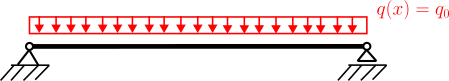
\includegraphics[width=0.7\linewidth]{files/Balken_Problem-ac2d1f8be068071b7e73a411e356e68c.png}
\caption[]{Statisch bestimmt gelagerter Balken mit konstanter Streckenlast}
\label{balken03}
\end{figure}

Für das dargestellte Beispiel eines statisch bestimmten Balkens mit konstanter Streckenlast lässt sich die Lösung der Verschiebung durch vierfache Integration der Differentialgleichung (\ref{balkendglsimple_2}) bestimmen. Die Lösung lautet:

\begin{equation}
\label{Balken_example_01}
EI w(x) =\frac{\ell^{3} q_{0} x}{24} - \frac{\ell q_{0} x^{3}}{12} + \frac{q_{0} x^{4}}{24}
\end{equation}

Über die Beziehungen:

\begin{align}
EI w'' & =-M(x) =  \frac{q_{0} x \left(\ell - x\right)}{2} \\
EI w'''' &= -Q(x) = q_{0} \left(\frac{\ell}{2} - x\right)
\end{align}
erhält man die Schnittgrö$\beta$en für das Biegemoment und die Querkraft.

Wir lösen nun dieses Problem mit der obigen Balken-FEM und vergleichen die Ergebnisse für die Durchbiegung und die Schnittgrö$\beta$en mit der analytischen Lösung.

\begin{figure}[!htbp]
\centering
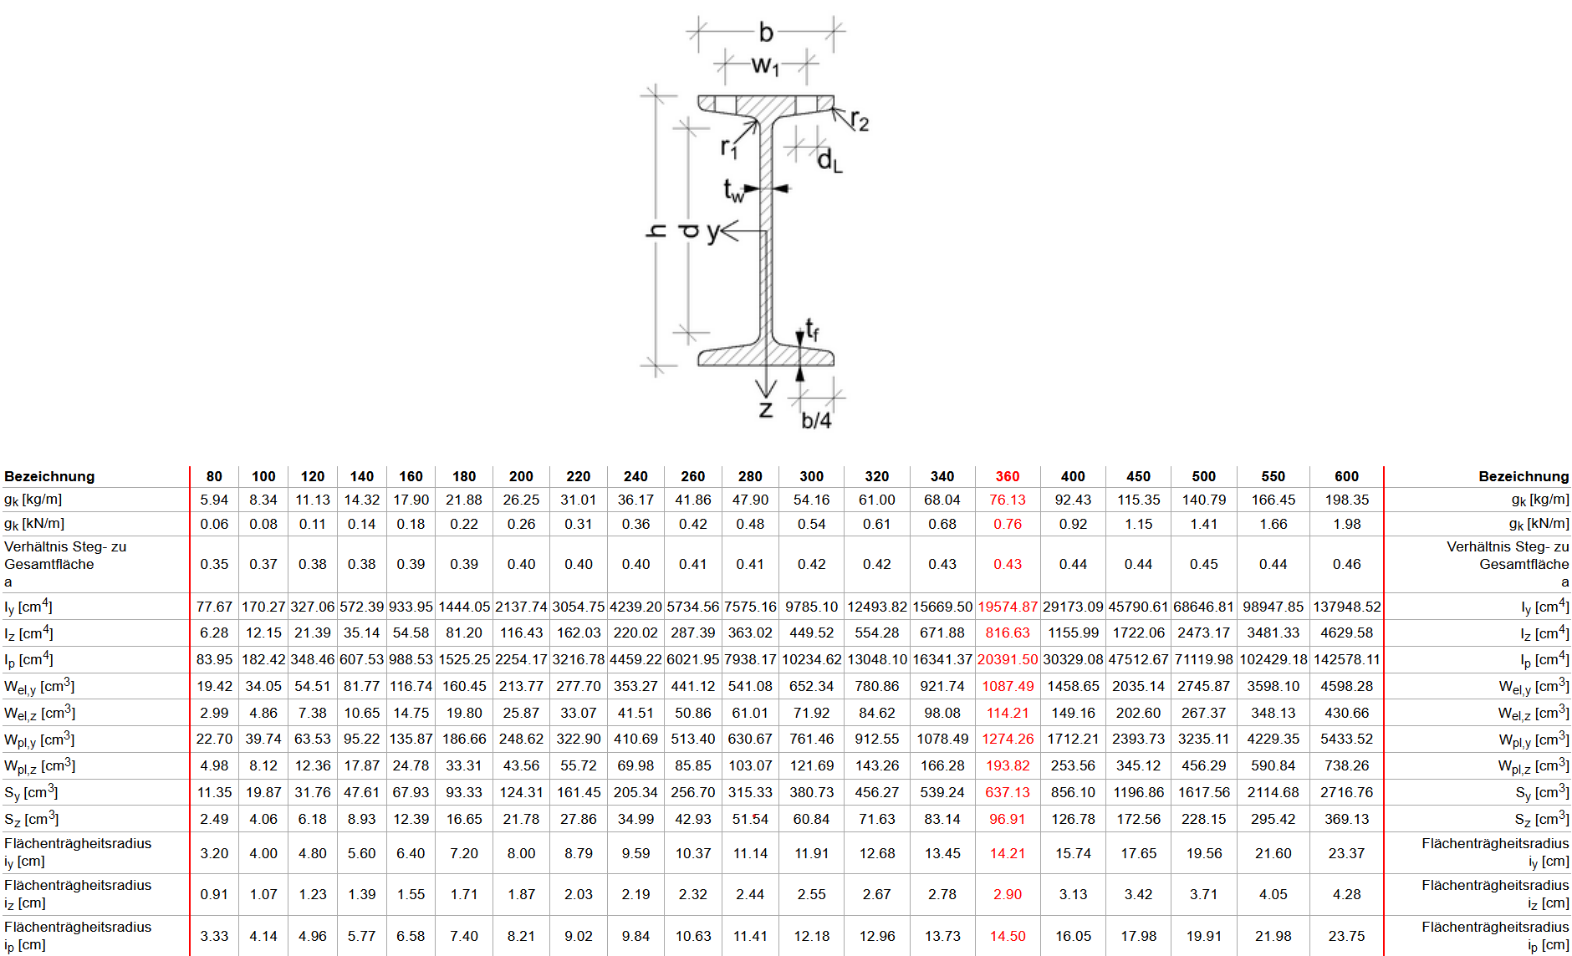
\includegraphics[width=0.8\linewidth]{files/Flächenträgheitsmome-3de341a2d042404c7134255287b1fae2.png}
\caption[]{Flächenträgheitsmomente für I-Profile nach DIN 1025-1:2009-04. \href{https://www.ezzat.org/de/Querschnittswerte/gewalzt/I/i.php}{ezzart.org}}
\label{FT}
\end{figure}

\paragraph{Ergebnisse der FEM-Berechnung}

\begin{figure}[!htbp]
\centering
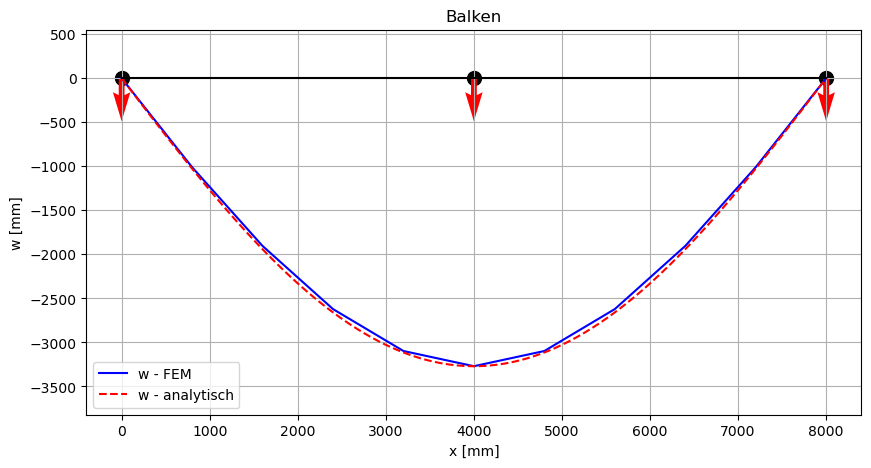
\includegraphics[width=0.625\linewidth]{files/Balken_FEM_01-a1f6ce8daf9026ef9f3fc80e01b3abcb.png}
\caption[]{Gegenüberstellung der analytischen Verschiebungslösung mit der FEM-Lösung.}
\label{BalkenFEM01}
\end{figure}

In Abbildung Figure~\ref{BalkenFEM01} ist die Verschiebungslösung der FEM mit der analytischen Lösung gegenübergestellt. Wir sehen, dass die FEM bereits mit nur 2 Elementen die analytische Lösung exakt trifft. Dies ist kein Zufall, sondern ein Ergebnis der Wahl der Formfunktionen und der Form der Randbedingungen.

Dies sollte jedoch nicht darüber hinwegtäuschen, dass die FEM-Lösung für das Schnittmoment und die Querkraft im Vergleich zur analytischen Lösung nicht so gut ist.

\begin{figure}[!htbp]
\centering
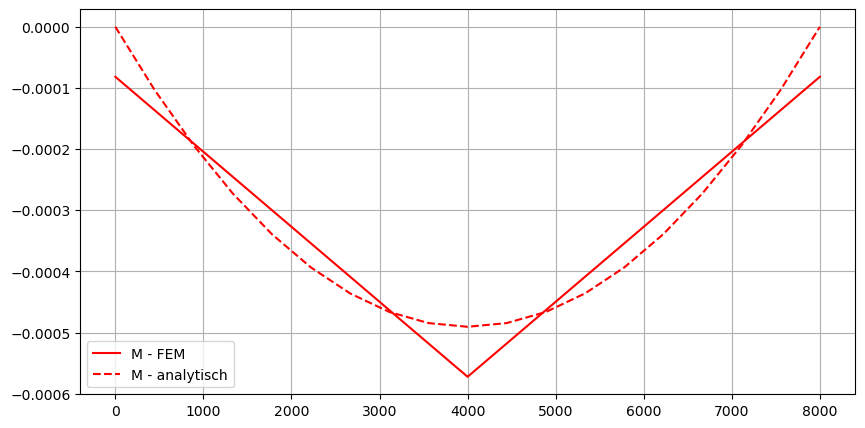
\includegraphics[width=0.625\linewidth]{files/Balken_FEM_02-4862ecf143a8bc5453774a7c198d23b3.png}
\caption[]{Gegenüberstellung der analytischen Lösung des Momentenverlaufs mit der FEM-Lösung.}
\label{BalkenFEM02}
\end{figure}

Das analytische Schnittmoment hat einen quadratischen Verlauf, während die FEM-Lösung linear ist. Dies führt zu einer Abweichung der FEM-Lösung von der analytischen Lösung.

\begin{figure}[!htbp]
\centering
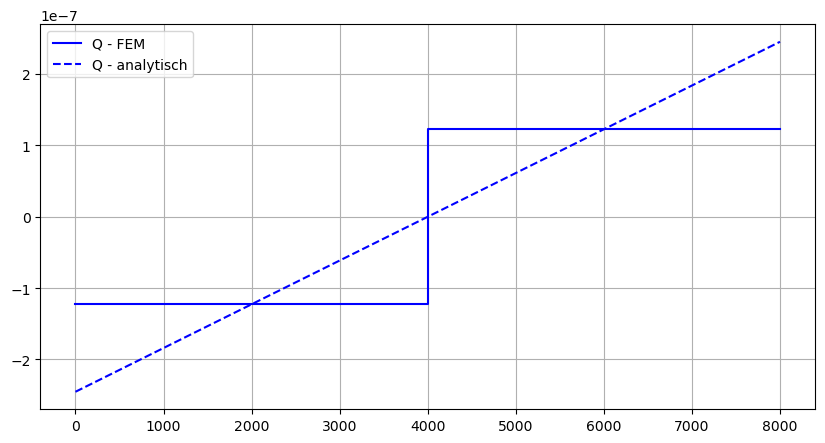
\includegraphics[width=0.625\linewidth]{files/Balken_FEM_03-c04f469fedcb8e67d9db06d983fbd4fd.png}
\caption[]{Gegenüberstellung der analytischen Lösung für den Querkraftverlauf mit der FEM-Lösung.}
\label{BalkenFEM03}
\end{figure}

Die Schnittkraft in der analytischen Lösung zeigt einen stückweise linearen Verlauf, während die FEM-Lösung konstant ist. Dies führt zu einer Abweichung der FEM-Lösung von der analytischen Lösung.

%  -+-+-+-+-+-+-AI-SPLIT

\paragraph{Konvergenz}

\begin{figure}[!htbp]
\centering
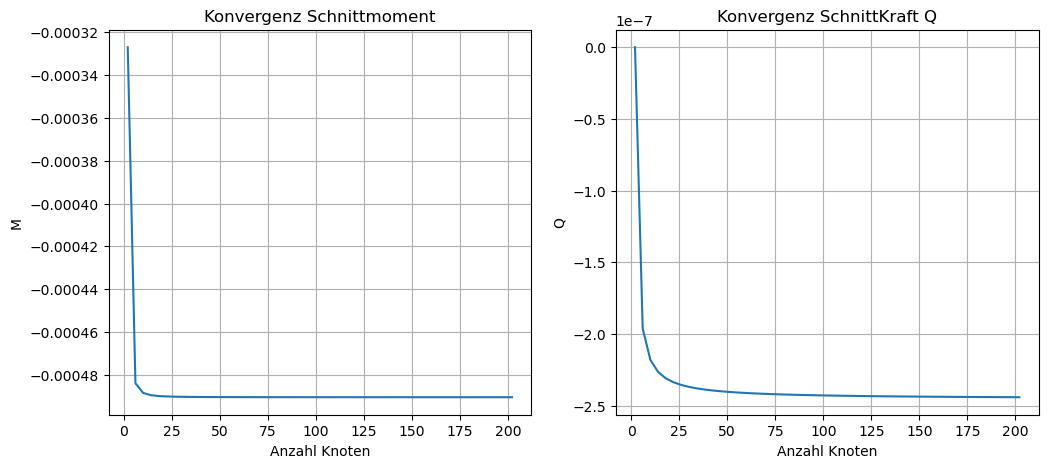
\includegraphics[width=0.75\linewidth]{files/Balken_FEM_04-5989c7a1d613e0755b5bf283d8b43fee.png}
\caption[]{Konvergenzverhalten der FEM-Lösung für das Schnittmoment und die Querkraft.}
\label{BalkenFEM04}
\end{figure}

Allgemein zeigt sich, dass die FEM-Lösung mit zunehmender Anzahl an Elementen gegen die analytische Lösung konvergiert. Dabei ist festzuhalten, dass die Konvergenz des Schnittmoments schneller ist als die Konvergenz der Querkraft. Dies zeigt sich auch im doppelt logarithmischen Diagramm Figure~\ref{BalkenFEM05}. Beide Kurven zeigen eine lineare Abhängigkeit, jedoch ist die Steigung der Konvergenzkurve für das Schnittmoment grö$\beta$er als die Steigung der Konvergenzkurve für die Querkraft.

\begin{figure}[!htbp]
\centering
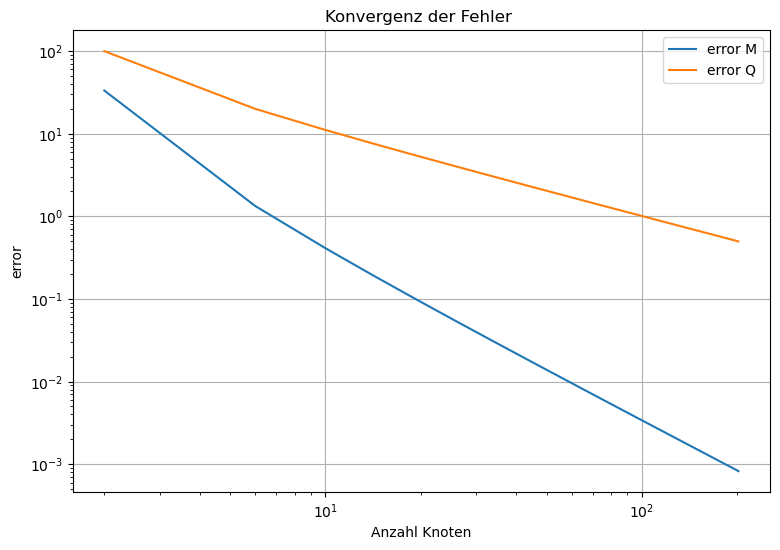
\includegraphics[width=0.75\linewidth]{files/Balken_FEM_05-696ae86f3f41368fe7073b08fecfddd0.png}
\caption[]{Konvergenzverhalten der FEM-Lösung für das Schnittmoment und die Querkraft im doppelt logarithmischen Diagramm.}
\label{BalkenFEM05}
\end{figure}

\paragraph{Interaktives Notebook}

Basierend auf der präsentierten Theorie wurde ein Jupyter Notebook erstellt. Dieses kann man ohne Systemvoraussetzungen im Browser ausführen:

Balken FEM for Binder \href{https://mybinder.org/v2/gh/steffenbeese/FEM\_I\_Notebooks/main?urlpath=\%2Fdoc\%2Ftree\%2FNotebook\_BalkenFEM.ipynb}{
\includegraphics[width=0.2\linewidth]{files/b77199e99a54e59b2e3c037c2cc90f21.pdf}
}

\begin{framed}
\textbf{Fragen zum Kapitel}\\
\textbf{Balken FEM}

\begin{itemize}
\item Welche physikalische Interpretation haben die Knotenfreiheitsgrade beim Balkenelement?


\item Wie gut ist die Lösung der Balken-FEM bzgl. der Verschiebungen im Vergleich zur analytischen Lösung?


\item Welche Aussage ist richtig:

\begin{itemize}
\item Das Schnittmoment ist linear im Element.
\item Die Schnittkraft ist linear im Element.
\item Die Verschiebung ist über die Elementgrenzen stetig.
\item Die Ableitung der Verschiebung ist über die Elementgrenzen stetig.
\end{itemize}
\end{itemize}
\end{framed}